\documentclass[12pt,a4paper]{article}

% ─── Page Layout ───────────────────────────────────────────────────────────────
\usepackage[a4paper, margin=0.8in, headheight=14pt]{geometry}

% ─── Fonts (XeLaTeX) ───────────────────────────────────────────────────────────
\usepackage{fontspec}
\usepackage{unicode-math}
\setmainfont{TeX Gyre Pagella}
\setmonofont[Scale=0.88]{TeX Gyre Cursor}
\setmathfont{Latin Modern Math}

% ─── Packages ──────────────────────────────────────────────────────────────────
\usepackage{xcolor}
\usepackage{colortbl}
\usepackage{titlesec}
\usepackage{enumitem}
\usepackage{tabularx}
\usepackage{booktabs}
\usepackage{array}
\usepackage{amsmath}
\usepackage{tikz}
\usetikzlibrary{shapes.geometric, arrows.meta, positioning, calc, fit, decorations.pathreplacing, patterns}
\usepackage{tcolorbox}
\tcbuselibrary{skins, breakable}
\usepackage{hyperref}
\usepackage{fancyhdr}
\usepackage{graphicx}
\usepackage{microtype}
\hyphenpenalty=10000
\exhyphenpenalty=10000
\sloppy
\usepackage{caption}
\usepackage{setspace}
\usepackage{multirow}
\usepackage{tocloft}

% ─── Q&A helper ────────────────────────────────────────────────────────────────
\newcommand{\Q}[1]{\textbf{#1}\par\noindent\ignorespaces}

% ─── Colour Palette ────────────────────────────────────────────────────────────
\definecolor{myred}{RGB}{196,30,58}
\definecolor{mydark}{RGB}{30,30,50}
\definecolor{mygreen}{RGB}{14,120,80}
\definecolor{myteal}{RGB}{0,130,140}
\definecolor{myamber}{RGB}{180,100,0}
\definecolor{mypurple}{RGB}{100,30,160}
\definecolor{mygray}{RGB}{246,247,249}
\definecolor{mgframe}{RGB}{180,185,200}
\definecolor{watermark}{RGB}{145,150,170}
\definecolor{hdrred}{RGB}{250,232,235}
\definecolor{hdrgreen}{RGB}{220,244,233}
\definecolor{hdrteal}{RGB}{220,242,244}
\definecolor{hdramber}{RGB}{253,242,215}
\definecolor{hdrpurple}{RGB}{238,228,255}
\definecolor{hdrgray}{RGB}{238,240,245}
\definecolor{rowalt}{RGB}{250,251,253}

% ─── Section Formatting ────────────────────────────────────────────────────────
\titleformat{\section}{\large\bfseries\color{myred}}{\thesection.}{0.5em}{}[\vspace{1pt}{\color{myred}\rule{\linewidth}{0.8pt}}]
\titleformat{\subsection}{\normalsize\bfseries\color{myteal}}{\thesubsection}{0.5em}{}
\titlespacing*{\section}{0pt}{18pt}{7pt}
\titlespacing*{\subsection}{0pt}{11pt}{4pt}

% ─── Paragraph ─────────────────────────────────────────────────────────────────
\setlength{\parindent}{0pt}
\setlength{\parskip}{4pt}

% ─── TOC Styling ───────────────────────────────────────────────────────────────
\renewcommand{\cfttoctitlefont}{\large\bfseries\color{myred}}
\renewcommand{\cftaftertoctitle}{\par\noindent{\color{myred}\rule{\linewidth}{0.8pt}}}
\setlength{\cftbeforetoctitleskip}{0pt}
\setlength{\cftaftertoctitleskip}{6pt}
\renewcommand{\cftsecfont}{\normalsize\bfseries\color{mydark}}
\renewcommand{\cftsecpagefont}{\normalsize\bfseries\color{mydark}}
\renewcommand{\cftsecleader}{\cftdotfill{\cftdotsep}}
\setlength{\cftbeforesecskip}{7pt}
\renewcommand{\cftsubsecfont}{\small\color{mydark}}
\renewcommand{\cftsubsecpagefont}{\small\color{mydark}}
\setlength{\cftbeforesubsecskip}{3pt}
\setlength{\cftsubsecindent}{1.4em}

% ─── Table helpers ─────────────────────────────────────────────────────────────
\renewcommand{\arraystretch}{1.45}
\setlength{\tabcolsep}{6pt}
\arrayrulecolor{mydark}
\newcolumntype{B}[1]{>{\small\bfseries\raggedright\arraybackslash}m{#1}}
\newcolumntype{Y}{>{\small\raggedright\arraybackslash}X}
\renewcommand{\tabularxcolumn}[1]{m{#1}}

% ─── Header / Footer ───────────────────────────────────────────────────────────
\pagestyle{fancy}
\fancyhf{}
\fancyhead[L]{\small\color{myred}\textbf{OE-EC803A}\;\color{mydark}--- Internet of Things}
\fancyhead[R]{\small\color{myteal}\textbf{Module 5 Notes}}
\fancyfoot[C]{\small\color{mydark}\thepage}
\fancyfoot[R]{\small\color{watermark}\textit{\copyright\ Biraj Sarkar}}
\renewcommand{\headrulewidth}{0.5pt}
\renewcommand{\footrulewidth}{0.3pt}

% ─── Hyperref ──────────────────────────────────────────────────────────────────
\hypersetup{colorlinks=true, linkcolor=myteal, urlcolor=myteal,
  pdfauthor={Biraj Sarkar}, pdftitle={OE-EC803A --- Module 5 Notes}}

% ─── tcolorbox styles ──────────────────────────────────────────────────────────
\tcbset{
  tikzbox/.style={colback=mygray, colframe=mgframe, boxrule=0.6pt, arc=4pt,
    left=8pt, right=8pt, top=6pt, bottom=6pt,
    colbacktitle=mgframe, coltitle=mydark, fonttitle=\small\bfseries},
  defbox/.style={colback=hdrgreen, colframe=mygreen, boxrule=0.8pt, arc=4pt,
    left=9pt, right=9pt, top=6pt, bottom=6pt,
    colbacktitle=mygreen, coltitle=white, fonttitle=\small\bfseries},
  formulabox/.style={colback=hdrteal, colframe=myteal, boxrule=0.8pt, arc=4pt,
    left=9pt, right=9pt, top=7pt, bottom=7pt,
    colbacktitle=myteal, coltitle=white, fonttitle=\small\bfseries},
  examplebox/.style={colback=hdramber, colframe=myamber, boxrule=0.8pt, arc=4pt,
    left=9pt, right=9pt, top=6pt, bottom=6pt,
    colbacktitle=myamber, coltitle=white, fonttitle=\small\bfseries},
  masonbox/.style={colback=hdrpurple, colframe=mypurple, boxrule=0.8pt, arc=4pt,
    left=9pt, right=9pt, top=6pt, bottom=6pt,
    colbacktitle=mypurple, coltitle=white, fonttitle=\small\bfseries},
  exambox/.style={colback=hdrpurple, colframe=mypurple, boxrule=1pt, arc=5pt,
    left=10pt, right=10pt, top=8pt, bottom=8pt,
    colbacktitle=mypurple, coltitle=white, fonttitle=\bfseries,
    breakable, title after break={\textbf{Frequently Asked / Viva Questions (contd.)}}}
}
\tcbset{breakable}

% ─── TikZ styles ───────────────────────────────────────────────────────────────
\tikzset{
  line/.style={draw, thick, color=mydark},
  arrow/.style={-Stealth, thick, color=mydark}
}

\begin{document}

% ═══════════════════════════════════════════════════════════════════════════════
% TITLE BLOCK
% ═══════════════════════════════════════════════════════════════════════════════
\begin{center}
  \hfill \textit{Exam-Ready Short Notes} \\
  \vspace{6pt}
  {\LARGE\bfseries\color{myred} OE-EC803A --- Internet of Things}\\[5pt]
  {\normalsize\color{mydark} Semester VIII \quad$\bullet$\quad 3L:0T:0P \quad$\bullet$\quad 3 Credits}\\[3pt]
  {\normalsize\color{myteal}\textbf{Module 5: Prototyping Online Components \& Embedded Programming}}\\[3pt]
  {\small\color{mydark} CGEC \;$|$\; B.Tech ECE (2023--27) \;$|$\; \textit{Biraj Sarkar}}
\end{center}
\vspace{2pt}
\noindent{\color{myred}\rule{\linewidth}{1.5pt}}
\vspace{2pt}

\hypersetup{linkcolor=mydark}
\tableofcontents
\hypersetup{linkcolor=myteal}
\newpage

% ===============================================================================
\section{Prototyping Online Components (APIs)}
% ===============================================================================

To connect physical hardware to cloud services, devices communicate with web application interfaces called APIs (Application Programming Interfaces).

\subsection{RESTful APIs}
\begin{tcolorbox}[defbox, title={REST API}]
  A \textbf{REST (Representational State Transfer) API} is an architectural style for network applications that uses standard HTTP requests to manage resources. Each resource is identified by a URL (e.g. `/devices/lamp1`) and manipulated using standard HTTP verbs.
\end{tcolorbox}
The primary HTTP verbs used in IoT APIs include:
\begin{itemize}[leftmargin=*, itemsep=2pt]
  \item \textbf{GET:} Retrieve the status/value of a sensor or actuator.
  \item \textbf{POST:} Create a new status log or register a new device.
  \item \textbf{PUT / PATCH:} Update configuration properties or toggle state.
  \item \textbf{DELETE:} Remove a device instance from the registry database.
\end{itemize}

Common HTTP response status codes returned by IoT APIs:
\begin{itemize}[leftmargin=*, itemsep=2.5pt]
  \item \textbf{200 OK:} Request succeeded (e.g. GET returned sensor reading).
  \item \textbf{201 Created:} Resource successfully created (e.g. POST registered a new device).
  \item \textbf{400 Bad Request:} Invalid syntax or malformed JSON payload.
  \item \textbf{401 Unauthorized:} Missing or invalid API key / authentication token.
  \item \textbf{404 Not Found:} Target device or resource URL does not exist.
  \item \textbf{500 Internal Server Error:} Server-side runtime database/connection failure.
\end{itemize}

Data is commonly formatted in \textbf{JSON (JavaScript Object Notation)} due to its low parsing overhead and human-readable, key-value structure:
\begin{verbatim}
{
  "device_id": "sensor_node_04",
  "temperature": 26.5,
  "status": "active"
}
\end{verbatim}
\subsection{Writing a New API (Backend Endpoint)}
Writing a new REST API endpoint involves setting up a server runtime (e.g. Node.js with Express or Python with Flask) that accepts incoming JSON payloads, processes them, and returns standard HTTP response codes.
\begin{tcolorbox}[examplebox, title={Express.js IoT Server-Side Logging API}]
  Below is a standard server-side Node.js script that listens for HTTP \texttt{POST} requests from IoT sensor nodes and saves the reading:
\begin{verbatim}
const express = require('express');
const app = express();
app.use(express.json()); // Parse JSON payloads

app.post('/api/telemetry', (req, res) => {
  const { device_id, temperature } = req.body;
  
  if (!device_id || temperature === undefined) {
    return res.status(400).json({ error: "Missing parameters" });
  }
  
  console.log(`Log from ${device_id}: ${temperature} C`);
  // (In production: Insert data into MongoDB or PostgreSQL database)
  
  res.status(201).json({ 
    message: "Data logged successfully", 
    timestamp: new Date() 
  });
});

app.listen(3000, () => console.log('IoT Server running on port 3000'));
\end{verbatim}
\end{tcolorbox}
\subsection{Real-Time Reactions: Polling vs. WebSockets}
IoT systems need to push real-time events (e.g., triggering an alarm).
\begin{itemize}[leftmargin=*, itemsep=3.5pt]
  \item \textbf{HTTP Polling:} The client periodically sends GET requests to the server (e.g., every 5 seconds) to check for updates. This generates significant network overhead and latency.
  \item \textbf{HTTP Long Polling:} The server holds the client's request open until new data is available, responding immediately, then closing the connection.
  \item \textbf{WebSockets:} Establishes a persistent, bi-directional TCP connection. Both client and server can send data packets at any time with minimal header overhead, enabling sub-millisecond real-time reactions.
\end{itemize}

\begin{tcolorbox}[tikzbox, title={HTTP Polling vs. WebSockets Communication Flow}]
\centering
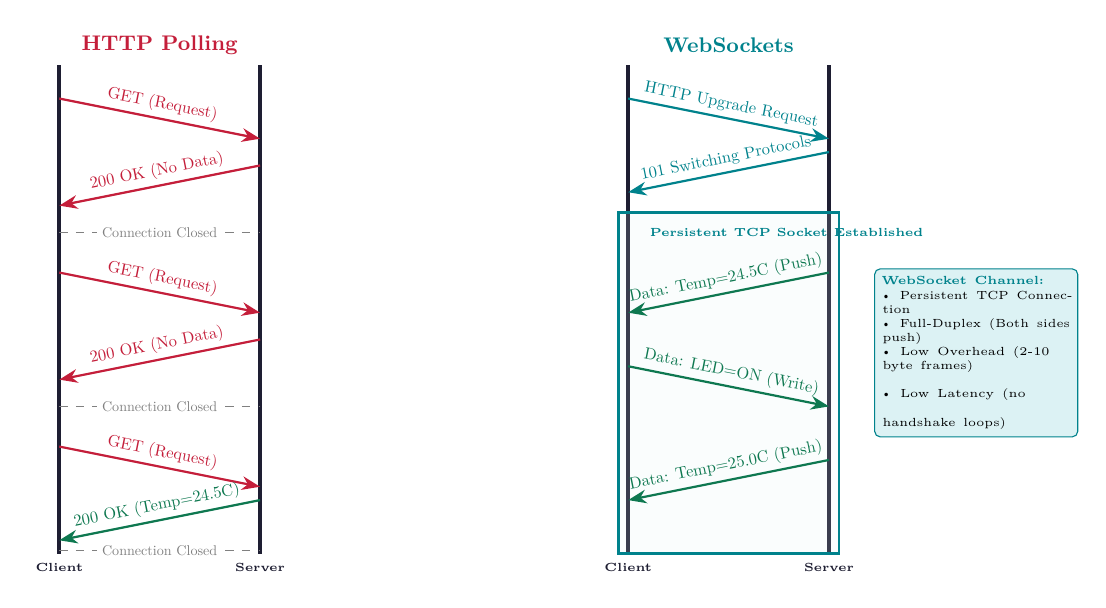
\begin{tikzpicture}[scale=0.85, transform shape]
  % ═══════════════════════════════════════════════════════════════════════════════
  % LEFT SIDE: HTTP POLLING (Wider spacing, sloped text labels)
  % ═══════════════════════════════════════════════════════════════════════════════
  \node[font=\small\bfseries\color{myred}] at (-6.0, 3.8) {HTTP Polling};
  \draw[line width=1.5pt, color=mydark] (-7.5, 3.5) -- (-7.5, -3.8) node[below, font=\tiny\bfseries] {Client};
  \draw[line width=1.5pt, color=mydark] (-4.5, 3.5) -- (-4.5, -3.8) node[below, font=\tiny\bfseries] {Server};

  % Exchange 1
  \draw[arrow, color=myred] (-7.5, 3.0) -- node[midway, above, sloped, scale=0.7] {GET (Request)} (-4.5, 2.4);
  \draw[arrow, color=myred] (-4.5, 2.0) -- node[midway, above, sloped, scale=0.7] {200 OK (No Data)} (-7.5, 1.4);
  \draw[dashed, color=gray] (-7.5, 1.0) -- (-4.5, 1.0) node[midway, fill=white, scale=0.6] {Connection Closed};

  % Exchange 2
  \draw[arrow, color=myred] (-7.5, 0.4) -- node[midway, above, sloped, scale=0.7] {GET (Request)} (-4.5, -0.2);
  \draw[arrow, color=myred] (-4.5, -0.6) -- node[midway, above, sloped, scale=0.7] {200 OK (No Data)} (-7.5, -1.2);
  \draw[dashed, color=gray] (-7.5, -1.6) -- (-4.5, -1.6) node[midway, fill=white, scale=0.6] {Connection Closed};

  % Exchange 3
  \draw[arrow, color=myred] (-7.5, -2.2) -- node[midway, above, sloped, scale=0.7] {GET (Request)} (-4.5, -2.8);
  \draw[arrow, color=mygreen] (-4.5, -3.0) -- node[midway, above, sloped, scale=0.7] {200 OK (Temp=24.5C)} (-7.5, -3.6);
  \draw[dashed, color=gray] (-7.5, -3.75) -- (-4.5, -3.75) node[midway, fill=white, scale=0.6] {Connection Closed};


  % ═══════════════════════════════════════════════════════════════════════════════
  % RIGHT SIDE: WEBSOCKETS (Wider spacing, side-aligned description box)
  % ═══════════════════════════════════════════════════════════════════════════════
  \node[font=\small\bfseries\color{myteal}] at (2.5, 3.8) {WebSockets};
  \draw[line width=1.5pt, color=mydark] (1.0, 3.5) -- (1.0, -3.8) node[below, font=\tiny\bfseries] {Client};
  \draw[line width=1.5pt, color=mydark] (4.0, 3.5) -- (4.0, -3.8) node[below, font=\tiny\bfseries] {Server};

  % Handshake (HTTP Upgrade)
  \draw[arrow, color=myteal] (1.0, 3.0) -- node[midway, above, sloped, scale=0.7] {HTTP Upgrade Request} (4.0, 2.4);
  \draw[arrow, color=myteal] (4.0, 2.2) -- node[midway, above, sloped, scale=0.7] {101 Switching Protocols} (1.0, 1.6);

  % Persistent Connection Channel Box
  \draw[draw=myteal, fill=hdrteal, fill opacity=0.15, line width=1pt] (0.85, 1.3) rectangle (4.15, -3.8);
  \node[right, font=\tiny\bfseries, color=myteal] at (1.2, 1.0) {Persistent TCP Socket Established};

  % Bidirectional Pushes
  \draw[arrow, color=mygreen] (4.0, 0.4) -- node[midway, above, sloped, scale=0.7] {Data: Temp=24.5C (Push)} (1.0, -0.2);
  \draw[arrow, color=mygreen] (1.0, -1.0) -- node[midway, above, sloped, scale=0.7] {Data: LED=ON (Write)} (4.0, -1.6);
  \draw[arrow, color=mygreen] (4.0, -2.4) -- node[midway, above, sloped, scale=0.7] {Data: Temp=25.0C (Push)} (1.0, -3.0);

  % WebSocket Features Box (Placed completely to the right to prevent overlap)
  \node[draw=myteal, fill=hdrteal, rounded corners=2pt, text width=2.8cm, align=left] at (6.2, -0.8) {
    \tiny
    \textbf{\color{myteal}WebSocket Channel:}\\
    • Persistent TCP Connection\\
    • Full-Duplex (Both sides push)\\
    • Low Overhead (2-10 byte frames)\\
    • Low Latency (no handshake loops)
  };
\end{tikzpicture}
\end{tcolorbox}

\subsection{Other Messaging Protocols}
\begin{itemize}[leftmargin=*, itemsep=2.5pt]
  \item \textbf{XMPP (Extensible Messaging and Presence Protocol):} XML-based instant messaging protocol. Heavy overhead but features strong built-in security and routing.
  \item \textbf{AMQP (Advanced Message Queuing Protocol):} An open standard queuing protocol designed for enterprise transaction messaging, providing high reliability.
\end{itemize}

% ===============================================================================
\section{Techniques for Writing Embedded Code}
% ===============================================================================

Microcontrollers are resource-constrained devices, requiring specialized programming practices.

\subsection{Memory Management \& Heap Fragmentation}
\begin{tcolorbox}[defbox, title={Heap Fragmentation}]
  \textbf{Heap Fragmentation} occurs when dynamic memory allocation (`malloc()` and `free()`) allocates and deallocates varying memory chunks over time, leaving small, unusable gaps in the heap. In microcontrollers with only a few kilobytes of RAM, this can eventually prevent large allocations, leading to program crashes.
\end{tcolorbox}
To prevent fragmentation, embedded code should:
\begin{itemize}[leftmargin=*, itemsep=2.5pt]
  \item Avoid dynamic memory (`new`, `malloc`, `String` objects).
  \item Prefer static global allocation (defining buffer arrays with fixed sizes at compile time) or stack-based local variables.
\end{itemize}

\subsection{Power Management and Battery Life Optimization}
Many IoT devices run on batteries, requiring strict power management:
\begin{itemize}[leftmargin=*, itemsep=3pt]
  \item \textbf{Active Mode:} CPU running at full clock speed, radio transmitting. Draws high current ($10\text{mA}$ to $150\text{mA}$).
  \item \textbf{Light Sleep:} CPU clock is gated/halted, RAM is preserved. Draws microamps ($100\mu\text{A}$ to $500\mu\text{A}$).
  \item \textbf{Deep Sleep:} CPU, RAM, and internal oscillators are completely shut down. Only an ultra-low-power Real-Time Clock (RTC) or external interrupt remains active. Draws nanoamps ($1\mu\text{A}$ to $15\mu\text{A}$). The device wakes up, reads sensors, transmits, and immediately sleeps again.
\end{itemize}

\begin{tcolorbox}[formulabox, title={Duty Cycling \& Battery Life}]
  \textbf{Duty Cycling} is the ratio of active time ($t_{\text{active}}$) to the total period ($T = t_{\text{active}} + t_{\text{sleep}}$):
  \begin{equation}
    D = \frac{t_{\text{active}}}{t_{\text{active}} + t_{\text{sleep}}}
  \end{equation}
  The average current draw ($I_{\text{avg}}$) is calculated as:
  \begin{equation}
    I_{\text{avg}} = D \cdot I_{\text{active}} + (1 - D) \cdot I_{\text{sleep}}
  \end{equation}
  Battery lifetime ($L$ in hours) for a battery with capacity $C$ (in mAh) is:
  \begin{equation}
    L = \frac{C}{I_{\text{avg}}}
  \end{equation}
\end{tcolorbox}

\begin{tcolorbox}[examplebox, title={Numerical Example: IoT Battery Life Calculation}]
  \textbf{Scenario:} An IoT sensor node wakes up once every $10$ minutes ($600\text{ seconds}$) for a duration of $2\text{ seconds}$ to read a sensor and transmit it via Wi-Fi.
  \begin{itemize}[leftmargin=*, itemsep=2.5pt]
    \item Active Current ($I_{\text{active}}$) = $80\text{ mA}$
    \item Sleep Current ($I_{\text{sleep}}$) = $15\ \mu\text{A} = 0.015\text{ mA}$
    \item Battery Capacity ($C$) = $2400\text{ mAh}$ (e.g. standard AA cells)
  \end{itemize}
  \textbf{Step 1: Calculate Duty Cycle ($D$)}
  \begin{equation}
    D = \frac{2\text{ s}}{600\text{ s}} = 0.00333\quad (0.33\%)
  \end{equation}
  \textbf{Step 2: Calculate Average Current ($I_{\text{avg}}$)}
  \begin{equation}
    I_{\text{avg}} = (0.00333 \cdot 80\text{ mA}) + ((1 - 0.00333) \cdot 0.015\text{ mA})
  \end{equation}
  \begin{equation}
    I_{\text{avg}} \approx 0.2667\text{ mA} + 0.0150\text{ mA} = 0.2817\text{ mA}
  \end{equation}
  \textbf{Step 3: Calculate Battery Lifetime ($L$)}
  \begin{equation}
    L = \frac{2400\text{ mAh}}{0.2817\text{ mA}} \approx 8519.7\text{ hours} \approx 355\text{ days}
  \end{equation}
  Thus, by employing aggressive duty cycling, a standard battery can sustain the node for approximately one full year despite its high $80\text{mA}$ active transmission current.
\end{tcolorbox}

\subsection{Embedded Debugging Techniques}
Debugging on microcontrollers is challenging because they lack screens.
\begin{itemize}[leftmargin=*, itemsep=3pt]
  \item \textbf{Serial Debugging:} Printing variable values to a host computer serial monitor (`Serial.println()`). Simple but introduces delay (timing bugs).
  \item \textbf{In-Circuit Emulation \& JTAG:} A hardware interface (Joint Test Action Group) that connects directly to the CPU core, allowing developers to set hardware breakpoints, inspect memory registers, and step through code line-by-line.
\end{itemize}

\newpage

% ═══════════════════════════════════════════════════════════════════════════════
% QUICK REVISION PAGE
% ═══════════════════════════════════════════════════════════════════════════════
\begin{center}
  {\large\bfseries\color{myred} Quick Revision — Module 5}\\[3pt]
  {\small\color{mydark} Online Components \& Embedded Programming $|$ OE-EC803A}
\end{center}
\noindent{\color{myred}\rule{\linewidth}{1.2pt}}
\vspace{8pt}

\begin{tcolorbox}[formulabox, title={\textbf{Key Formulas and Metrics at a Glance}}]
\renewcommand{\arraystretch}{1.35}
\begin{tabularx}{\linewidth}{B{5.0cm} X}
  Duty Cycle & $D = \dfrac{t_{\text{active}}}{t_{\text{active}} + t_{\text{sleep}}} \quad (\text{ratio of active execution time})$ \\[4pt]
  Average Current & $I_{\text{avg}} = D \cdot I_{\text{active}} + (1 - D) \cdot I_{\text{sleep}} \quad (\text{power profile})$ \\[4pt]
  Battery Lifetime & $L = \dfrac{\text{Battery Capacity (mAh)}}{I_{\text{avg}} \text{ (mA)}} \quad (\text{operation hours})$
\end{tabularx}
\end{tcolorbox}

\vspace{6pt}

\begin{tcolorbox}[defbox, title={\textbf{One-Line Definitions}}]
\begin{itemize}[leftmargin=*, itemsep=3pt, topsep=0pt]
  \item \textbf{REST:} A stateless web architectural style that relies on standard HTTP methods (GET/POST).
  \item \textbf{WebSocket:} A persistent, full-duplex TCP socket connection for real-time web communication.
  \item \textbf{Duty Cycling:} The practice of powering down the device CPU and radio for periodic sleep intervals.
  \item \textbf{Deep Sleep:} The lowest power state of an MCU, turning off all internal blocks except the RTC wakeup timer.
  \item \textbf{JTAG:} A hardware port standard used for direct in-circuit programming, testing, and debugging.
\end{itemize}
\end{tcolorbox}

\vspace{6pt}

\begin{tcolorbox}[exambox, title={\textbf{Frequently Asked / Viva Questions}}]
\begin{enumerate}[leftmargin=*, topsep=0pt, label=\textbf{Q\arabic*.}, itemsep=6pt]
  \item \Q{Why is dynamic memory allocation (`malloc`) highly discouraged in microcontroller code?}
        Microcontrollers have extremely limited RAM (often a few kilobytes) and no virtual memory management. Repeated allocations and deallocations leave small gaps of unused memory on the heap (heap fragmentation). Eventually, a request for a contiguous memory block fails, causing a system crash.
        
  \item \Q{Compare HTTP Polling and WebSockets for real-time sensor updates.}
        HTTP Polling requires the client to repeatedly send new request handshakes and headers, creating heavy network congestion and latency. WebSockets establishes a single persistent TCP connection, enabling bi-directional, real-time message streams with minimal packet overhead.
        
  \item \Q{Calculate the average current and battery life of an IoT node with a $1000\text{mAh}$ battery. It draws $100\text{mA}$ for $2$ seconds when active, and $10\mu\text{A}$ ($0.01\text{mA}$) for $58$ seconds during sleep.}
        (1) Total Period $T = 2 + 58 = 60$ seconds. (2) Duty Cycle $D = 2 / 60 = 0.0333$ ($3.33\%$). (3) Average Current $I_{\text{avg}} = (0.0333 \times 100) + (0.9667 \times 0.01) = 3.33 + 0.0097 \approx 3.34\text{mA}$. (4) Lifetime $L = 1000 / 3.34 \approx 299.4$ hours ($\approx 12.5$ days).
        
  \item \Q{What occurs during deep sleep in an ESP8266 or ESP32 microcontroller?}
        During deep sleep, the CPU, RAM, and internal Wi-Fi radio are completely powered off. The only part of the chip that remains powered is the low-power RTC timer and select GPIO wake pins. The CPU must re-initialize (reboot) from scratch when waking up.
        
  \item \Q{What is a REST API HTTP POST request used for in IoT?}
        A POST request is used to push data from the client to the server, creating a new database record (e.g., posting a new temperature reading log at `/api/v1/telemetry`).
        
  \item \Q{Explain the JTAG debug interface.}
        JTAG is a hardware debugging protocol. It uses dedicated physical pins on the microcontroller to interface directly with the internal processor tap, allowing developers to halt CPU execution, step through commands, and read register states.
        
  \item \Q{What is JSON, and why is it preferred over XML in IoT applications?}
        JSON is a lightweight key-value text format for representing structured data. It has a much smaller character count than XML (no closing tags), which saves bandwidth, and requires significantly less CPU memory and time to parse.
        
  \item \Q{How does duty cycling extend device battery life?}
        Sensors rarely need to transmit data continuously. By sleeping for $99\%$ of the time and only waking up for a few seconds to sample and transmit data, the average current draw is reduced to microamps, extending battery life from days to years.
\end{enumerate}
\end{tcolorbox}

\vspace{6pt}

\begin{tcolorbox}[tikzbox, title={\textbf{Comparison Snapshot}}]
\textbf{HTTP Polling vs. WebSockets:}\par\vspace{6pt}\noindent
{\renewcommand{\arraystretch}{1.35}%
\begin{tabularx}{\linewidth}{|B{3.2cm}|Y|Y|}
\hline
\textbf{Feature} & \textbf{HTTP Polling} & \textbf{WebSockets} \\
\hline
Connection Type & Temporary; opened and closed per request. & Persistent; remains open until closed. \\
\hline
Communication & Half-duplex (client pull only). & Full-duplex (bi-directional push/pull). \\
\hline
Network Overhead & High (repeats TCP handshakes and HTTP headers). & Minimal (small frame header of 2-10 bytes). \\
\hline
Real-Time Latency & High (depends on polling frequency). & Extremely Low (sub-millisecond). \\
\hline
Best Use Case & Static data dashboards. & Real-time alerts, remote live control. \\
\hline
\end{tabularx}}
\end{tcolorbox}

\end{document}
